\section{Figures}
\label{app:figures}

Figures~\ref{fig:coverage} to \ref{fig:candidates} are the exploratory analysis,
drawn by notebooks 01--04; Figures~\ref{fig:ladder} to \ref{fig:pilot} are
drawn by \code{src/figures\_phase2.py} from the same CSV tables the body's
numbers come from, so a figure cannot disagree with a table;
Figures~\ref{fig:app-predict} to \ref{fig:app-card} are the deployed
application.

\begin{figure}[htbp]
  \centering
  \includegraphics[width=\linewidth]{fig01_coverage_quality.pdf}
  \caption{(a) Monthly order volume. The pilot period before 2017 contributes 326
  orders in total and is excluded from the analysis window. (b) Missingness by
  column: structural rather than random, dominated by orders that never reached
  the customer.}
  \label{fig:coverage}
\end{figure}

\begin{figure}[htbp]
  \centering
  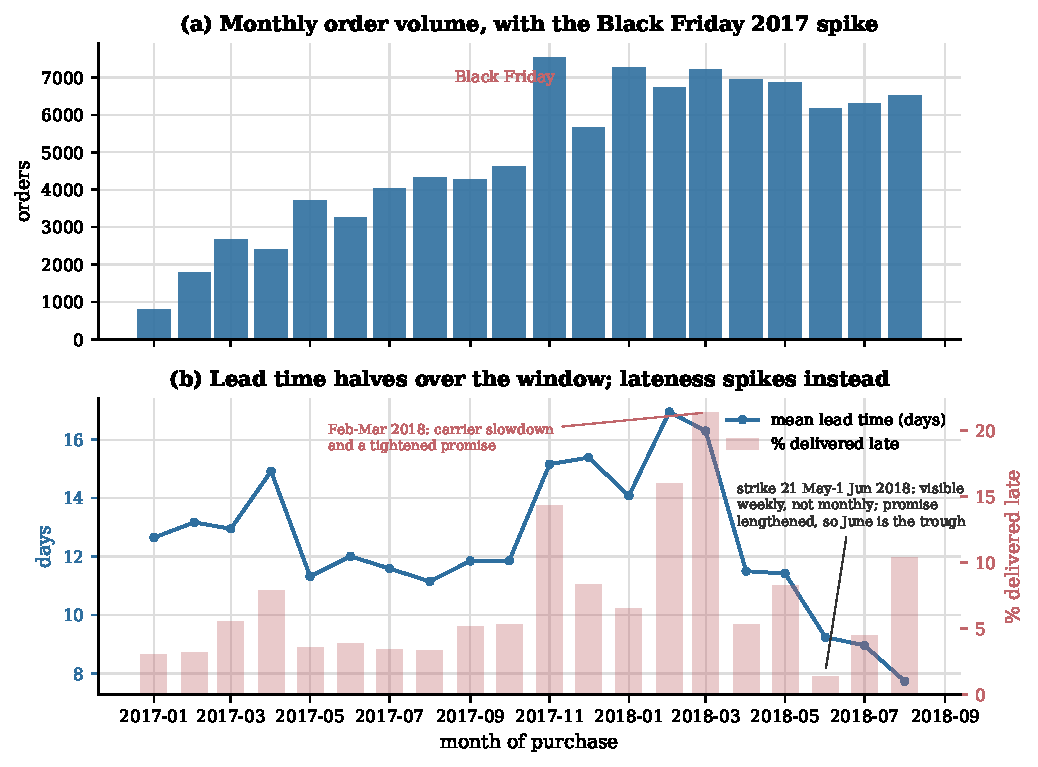
\includegraphics[width=\linewidth]{fig02_volume_drift.pdf}
  \caption{(a) Order volume with the Black Friday 2017 spike. (b) The central
  temporal finding: mean delivery lead time halves across the window (line, left
  axis) while the late rate is volatile rather than trending (bars, right axis).
  The spikes are Black Friday (November 2017) and February--March 2018, a
  carrier-side slowdown that coincided with a tightened promise. The truckers'
  strike of 21 May--1 June 2018 is not visible at monthly resolution
  (Section~\ref{sec:eda-lateness}).}
  \label{fig:volume}
\end{figure}

\begin{figure}[htbp]
  \centering
  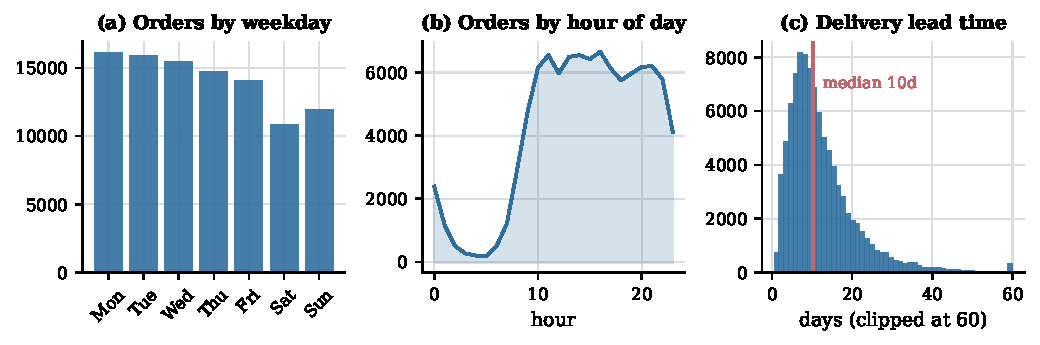
\includegraphics[width=\linewidth]{fig03_rhythm.pdf}
  \caption{Purchase rhythm and the lead-time distribution. Ordering is
  weekday-heavy and peaks at 16:00; lead time is right-skewed with a median of
  10.2 days and a long tail.}
  \label{fig:rhythm}
\end{figure}

\begin{figure}[htbp]
  \centering
  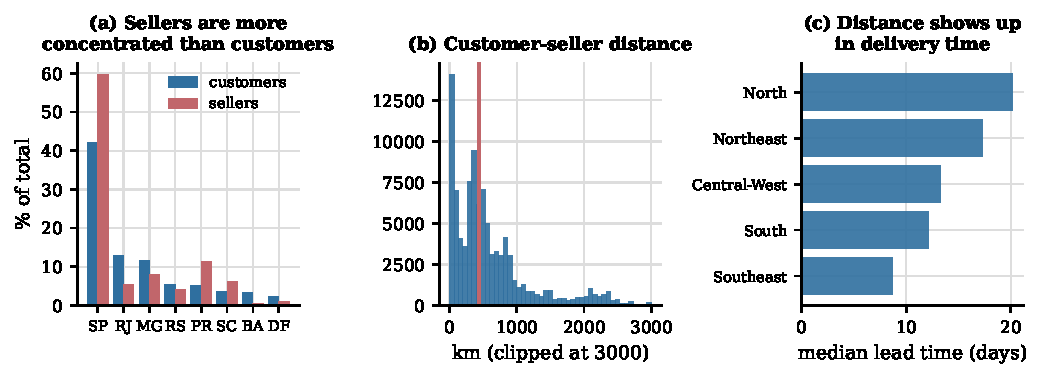
\includegraphics[width=\linewidth]{fig04_geography.pdf}
  \caption{(a) Sellers are far more concentrated in S\~{a}o Paulo than customers
  are, so most orders must cross the country. (b) Customer--seller distance.
  (c) That distance shows up directly in regional delivery times.}
  \label{fig:geography}
\end{figure}

\begin{figure}[htbp]
  \centering
  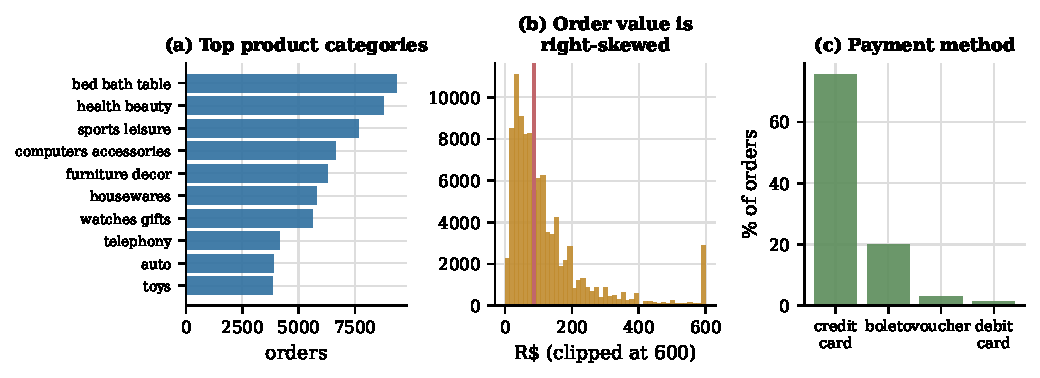
\includegraphics[width=\linewidth]{fig05_products_money.pdf}
  \caption{(a) Demand is long-tailed across 74 categories. (b) Order value is
  strongly right-skewed. (c) Credit card dominates, usually in instalments.}
  \label{fig:products}
\end{figure}

\begin{figure}[htbp]
  \centering
  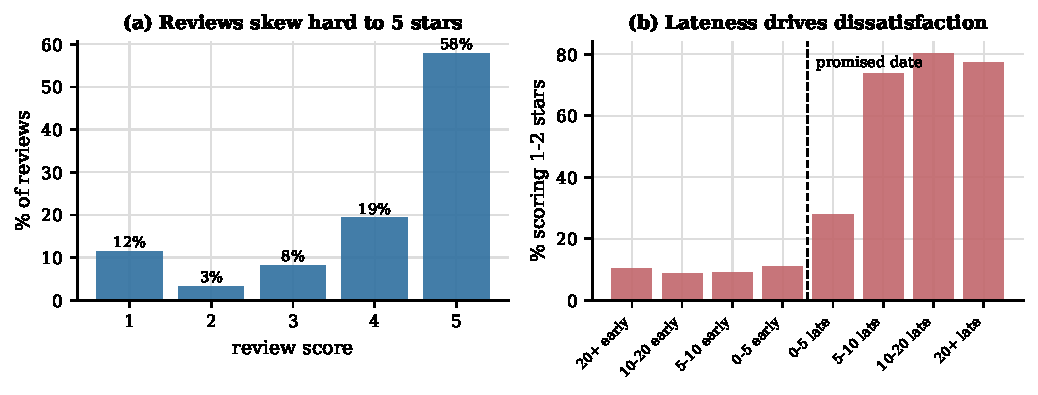
\includegraphics[width=\linewidth]{fig06_reviews_delivery.pdf}
  \caption{(a) Reviews are severely imbalanced towards five stars. (b) The
  strongest relationship in the dataset: the 1--2 star rate rises monotonically
  with lateness, from 9.2\% for on-time orders to 54.0\% for late ones.}
  \label{fig:reviews}
\end{figure}

\begin{figure}[htbp]
  \centering
  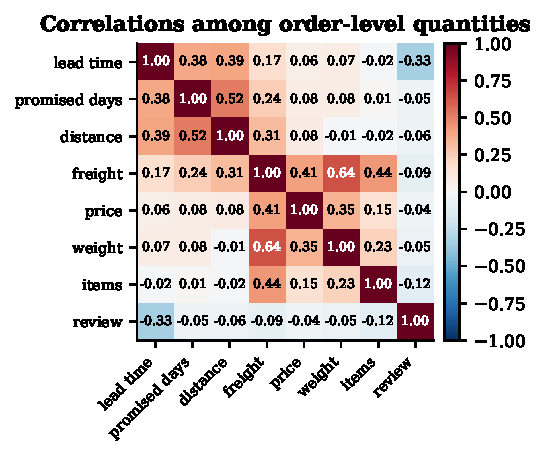
\includegraphics[width=0.62\linewidth]{fig07_correlations.pdf}
  \caption{Correlations among order-level quantities. Distance and the platform's
  own promise are the strongest checkout-time correlates of lead time; the
  review score moves with lead time and not with price.}
  \label{fig:correlations}
\end{figure}

\begin{figure}[htbp]
  \centering
  \includegraphics[width=0.58\linewidth]{fig08_leakage.pdf}
  \caption{What one forbidden column is worth. Adding the realised delivery time
  to the late-delivery model takes ROC-AUC from 0.589 to 1.000 --- the model is
  reading the answer, not predicting it.}
  \label{fig:leakage}
\end{figure}

\begin{figure}[htbp]
  \centering
  \includegraphics[width=\linewidth]{fig09_candidates.pdf}
  \caption{Candidate comparison from the scoping phase. (a) PR-AUC against the
  no-skill floor for each candidate and prediction moment. (b) Lead-time MAE:
  the platform's own promise is worse than a constant. (c) Raw accuracy flatters
  every imbalanced target; balanced accuracy does not.}
  \label{fig:candidates}
\end{figure}

\begin{figure}[htbp]
  \centering
  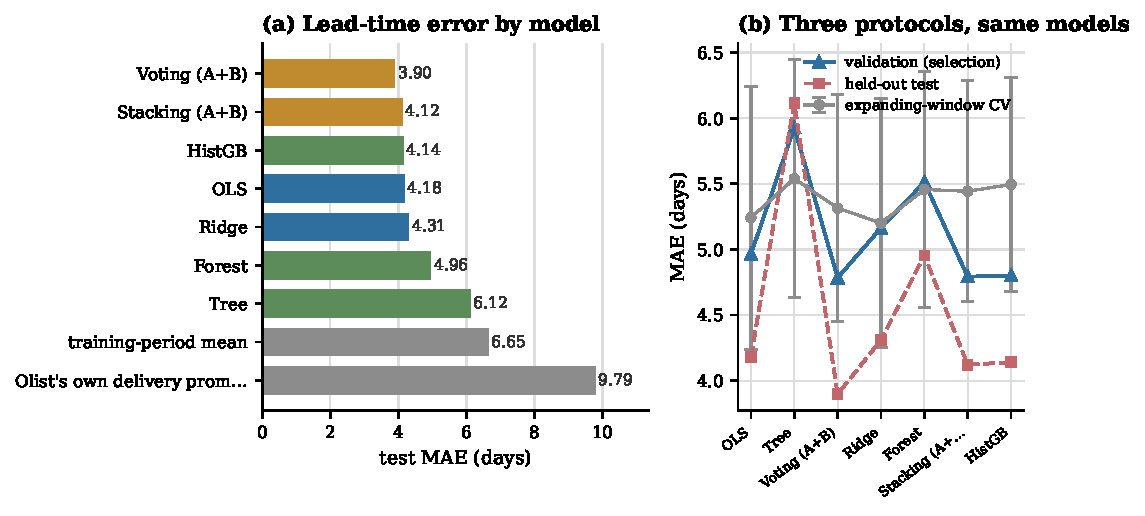
\includegraphics[width=\linewidth]{fig10_regression_ladder.pdf}
  \caption{Lead-time error by model, and the same models under three protocols.
  Panel (b) is the argument of Section~\ref{sec:cv}: expanding-window
  cross-validation does not order the candidates the way the validation period
  and the forward window --- which agree with each other --- do.}
  \label{fig:ladder}
\end{figure}

\begin{figure}[htbp]
  \centering
  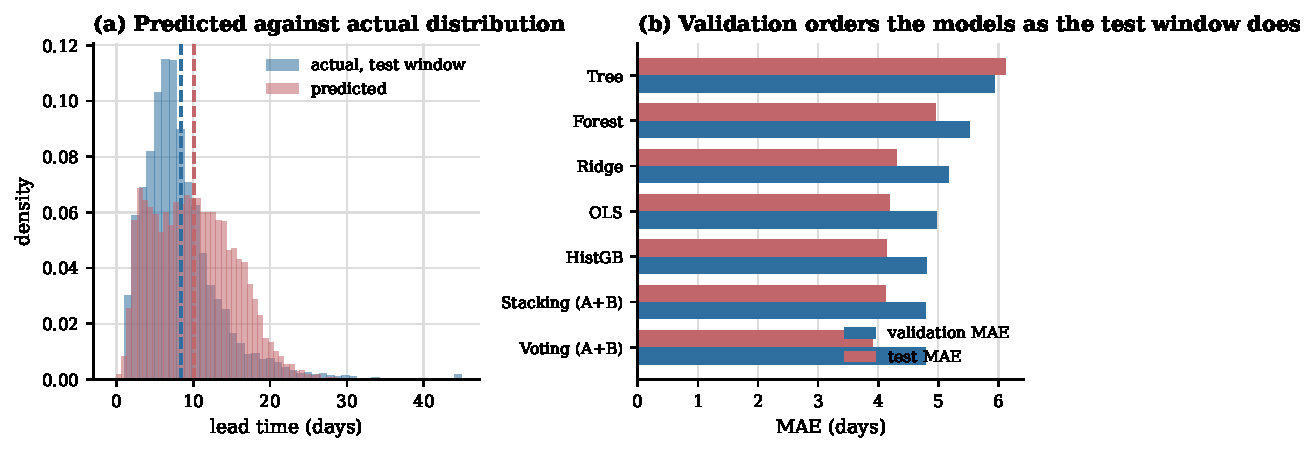
\includegraphics[width=\linewidth]{fig19_extrapolation.pdf}
  \caption{Why blending a linear model with a boosted one helps under drift. A
  tree cannot predict outside the range of the targets it was fitted on; lead
  times in the test window are systematically shorter than anything common in
  training. Panel (b) shows the validation period ordering the models as the test
  window does.}
  \label{fig:extrap}
\end{figure}

\begin{figure}[htbp]
  \centering
  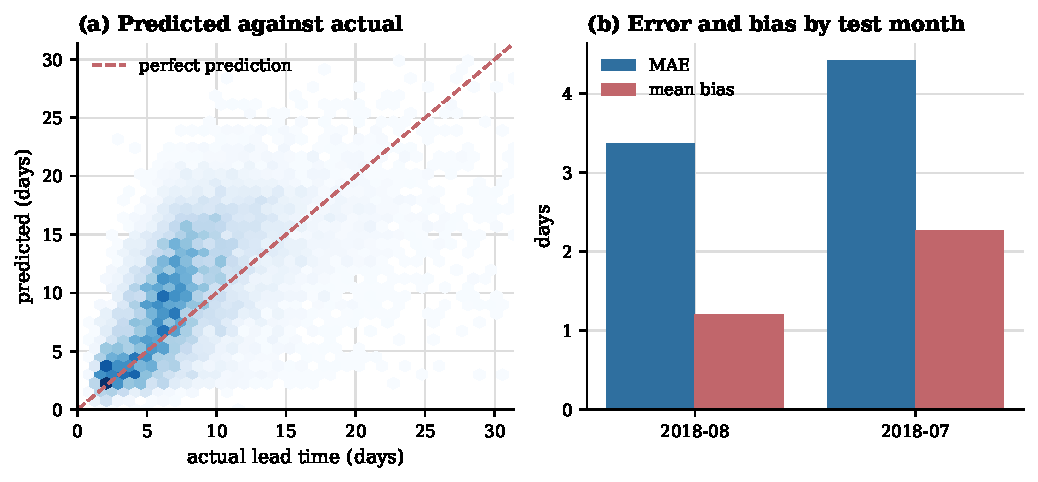
\includegraphics[width=\linewidth]{fig11_regression_residuals.pdf}
  \caption{Where the regression is wrong. The bias in panel (b) is positive in
  both test months: a model fitted on a slower past over-predicts how long a
  parcel will take.}
  \label{fig:resid}
\end{figure}

\begin{figure}[htbp]
  \centering
  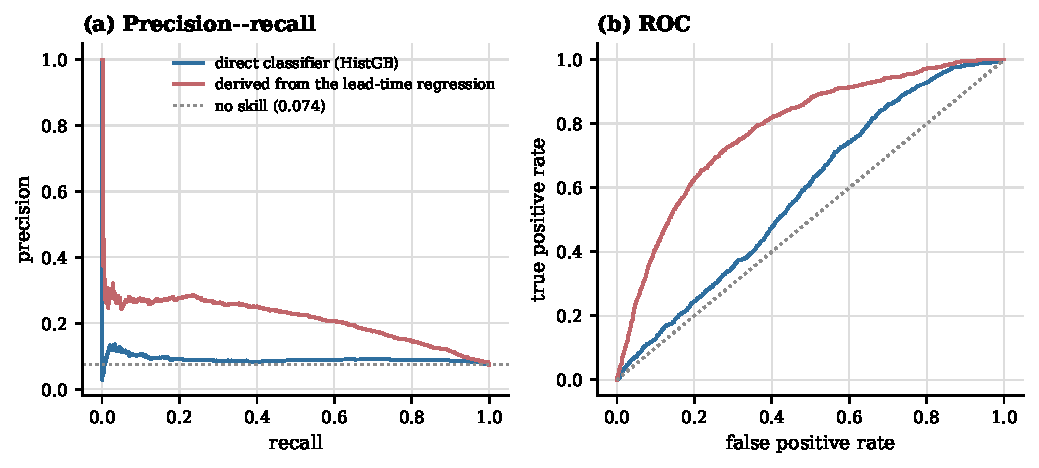
\includegraphics[width=\linewidth]{fig12_late_routes.pdf}
  \caption{Problem 1B. The flag derived from the lead-time regression against the
  best purpose-built classifier, on the forward test window.}
  \label{fig:routes}
\end{figure}

\begin{figure}[htbp]
  \centering
  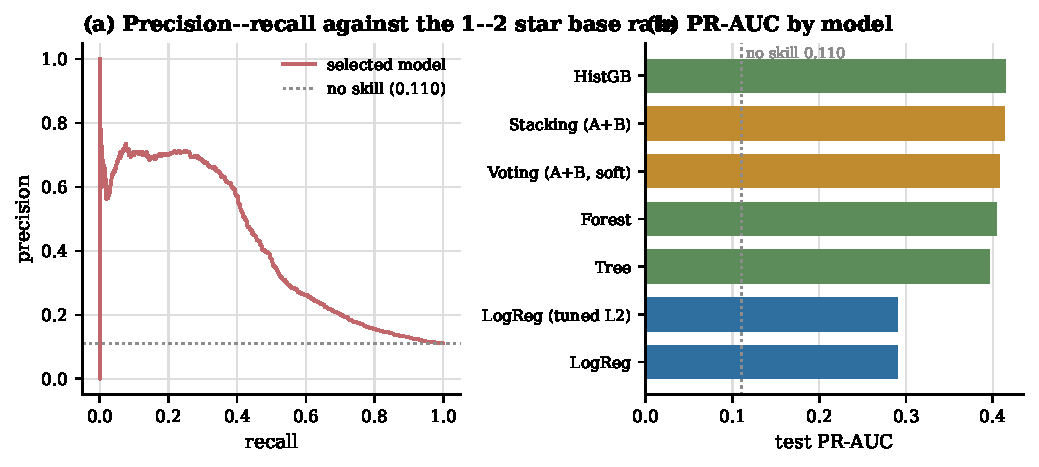
\includegraphics[width=\linewidth]{fig13_low_review.pdf}
  \caption{Problem 2 against its no-skill floor, and PR-AUC by model. Most of the
  achievable signal is already available from a single depth-limited tree.}
  \label{fig:lowreview}
\end{figure}

\begin{figure}[htbp]
  \centering
  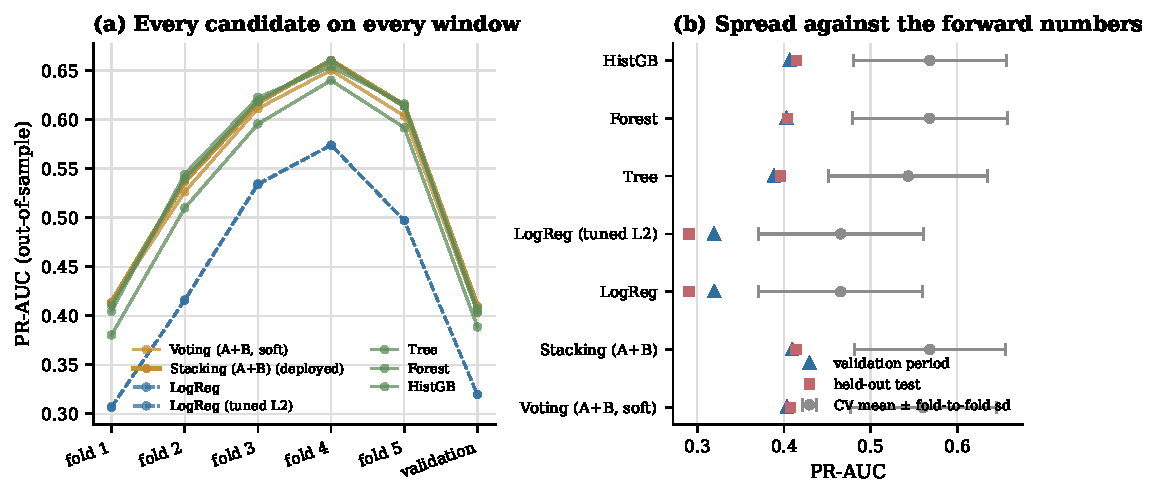
\includegraphics[width=\linewidth]{fig22_cv_folds.pdf}
  \caption{Fold-to-fold variation of every Problem 2 candidate
  (Table~\ref{tab:cvfolds}). (a) Each candidate's PR-AUC on the five expanding
  folds and the validation period: the windows move together, because their
  difficulty differs far more than the candidates do. (b) The cross-validated
  mean with its fold-to-fold standard deviation beside the validation and test
  scores: the spread is about 0.09 against a gap of under 0.001 between the best
  candidates.}
  \label{fig:cvfolds}
\end{figure}

\begin{figure}[htbp]
  \centering
  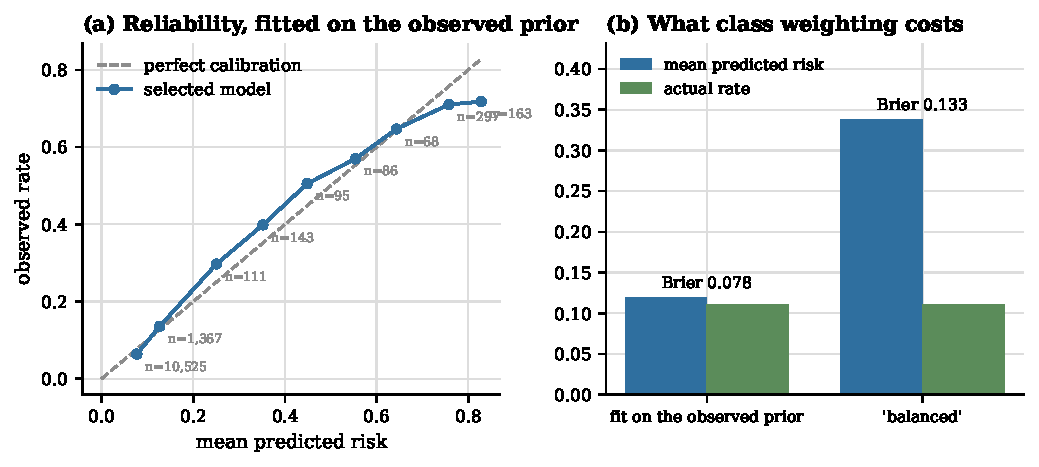
\includegraphics[width=\linewidth]{fig14_calibration.pdf}
  \caption{Calibration, and what class weighting costs. Weighting the loss leaves
  ranking unchanged and inflates mean predicted risk threefold against the actual
  rate.}
  \label{fig:calibration}
\end{figure}

\begin{figure}[htbp]
  \centering
  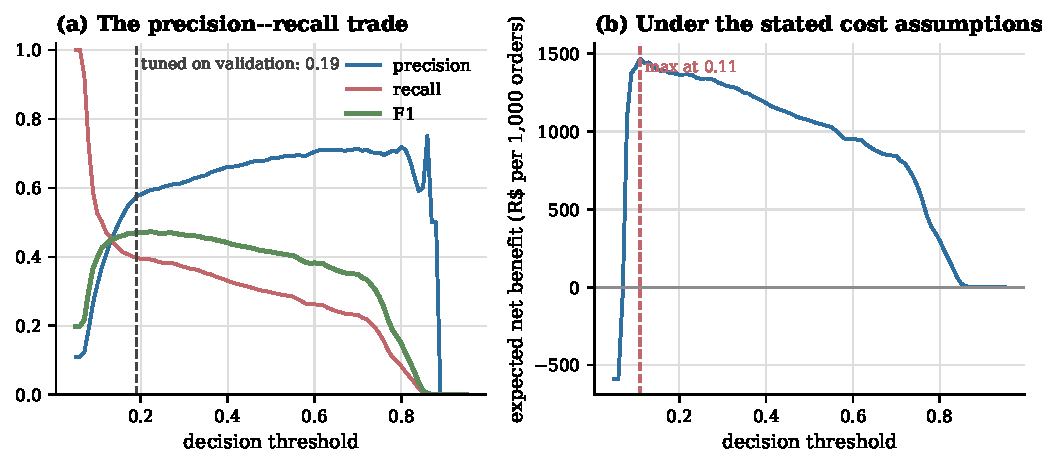
\includegraphics[width=\linewidth]{fig15_threshold_cost.pdf}
  \caption{Choosing the operating point for the review model, and what it is
  worth under the stated cost assumptions.}
  \label{fig:threshold}
\end{figure}

\begin{figure}[htbp]
  \centering
  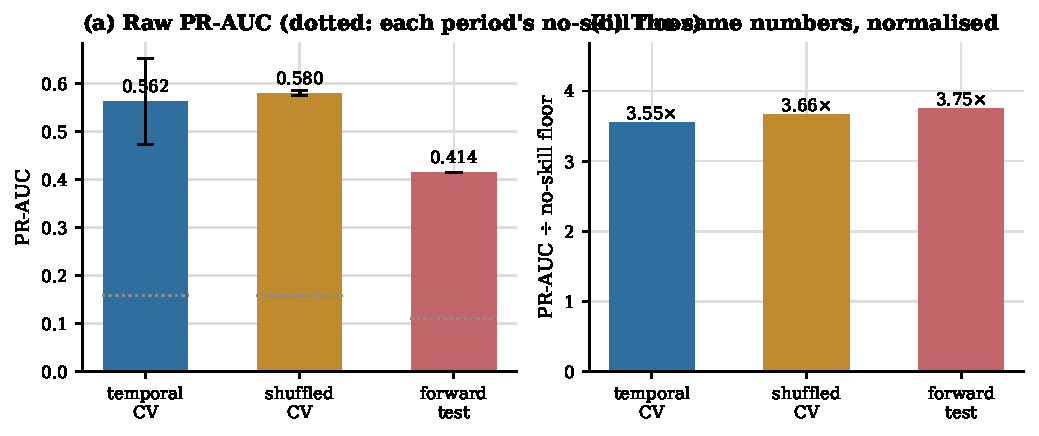
\includegraphics[width=\linewidth]{fig16_cv_protocol.pdf}
  \caption{One model, three protocols. Raw average precision disagrees across
  periods; divided by each period's no-skill floor the three agree to within 0.2
  of a multiple.}
  \label{fig:protocol}
\end{figure}

\begin{figure}[htbp]
  \centering
  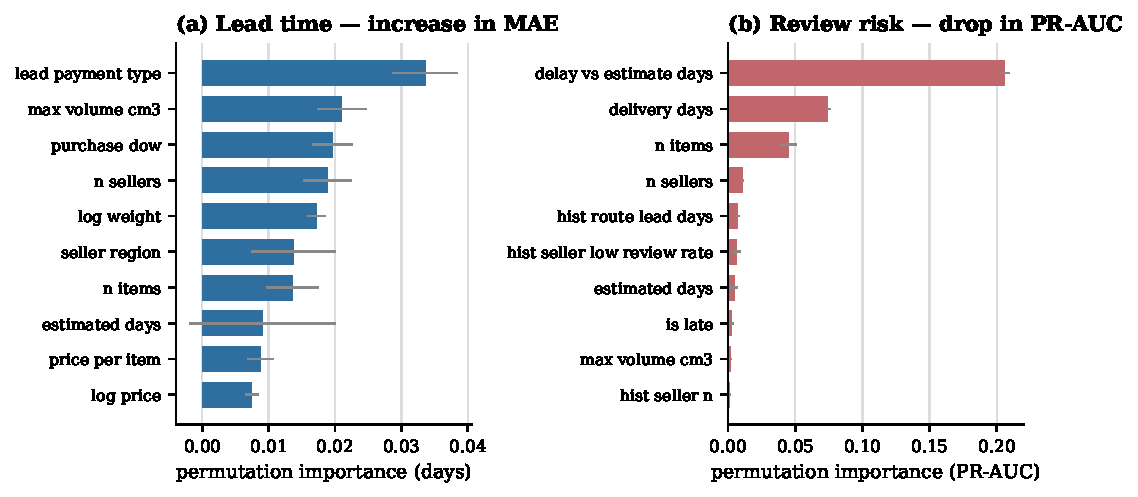
\includegraphics[width=\linewidth]{fig17_importance.pdf}
  \caption{Permutation importance on the test window. The review model rests on
  two features; the lead-time model on none in particular, which is a property of
  correlated predictors as much as of the model.}
  \label{fig:importance}
\end{figure}

\begin{figure}[htbp]
  \centering
  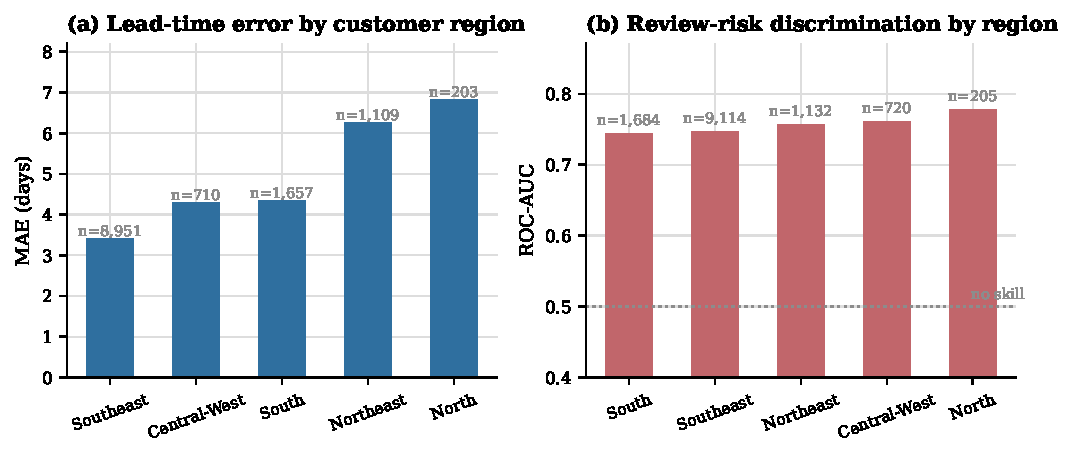
\includegraphics[width=\linewidth]{fig18_segments.pdf}
  \caption{Performance by customer region. The review model is stable across all
  five; the regression is not, and degrades exactly where deliveries are
  longest.}
  \label{fig:segments}
\end{figure}

\begin{figure}[htbp]
  \centering
  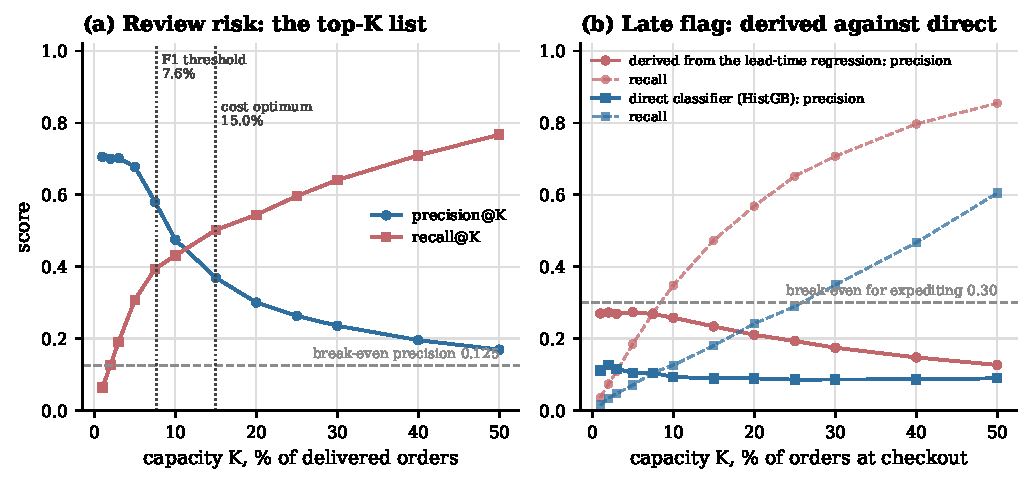
\includegraphics[width=\linewidth]{fig20_capacity.pdf}
  \caption{Precision and recall when only the top $K$ can be acted on
  (Section~\ref{sec:results-capacity}). (a) The review-risk list, with the
  report's two threshold operating points placed on the capacity axis; precision
  stays above the break-even at every capacity. (b) The late flag: the derived
  route beats the direct classifier at every $K$ and never reaches the
  break-even an expensive expedite would need.}
  \label{fig:capacity}
\end{figure}

\begin{figure}[htbp]
  \centering
  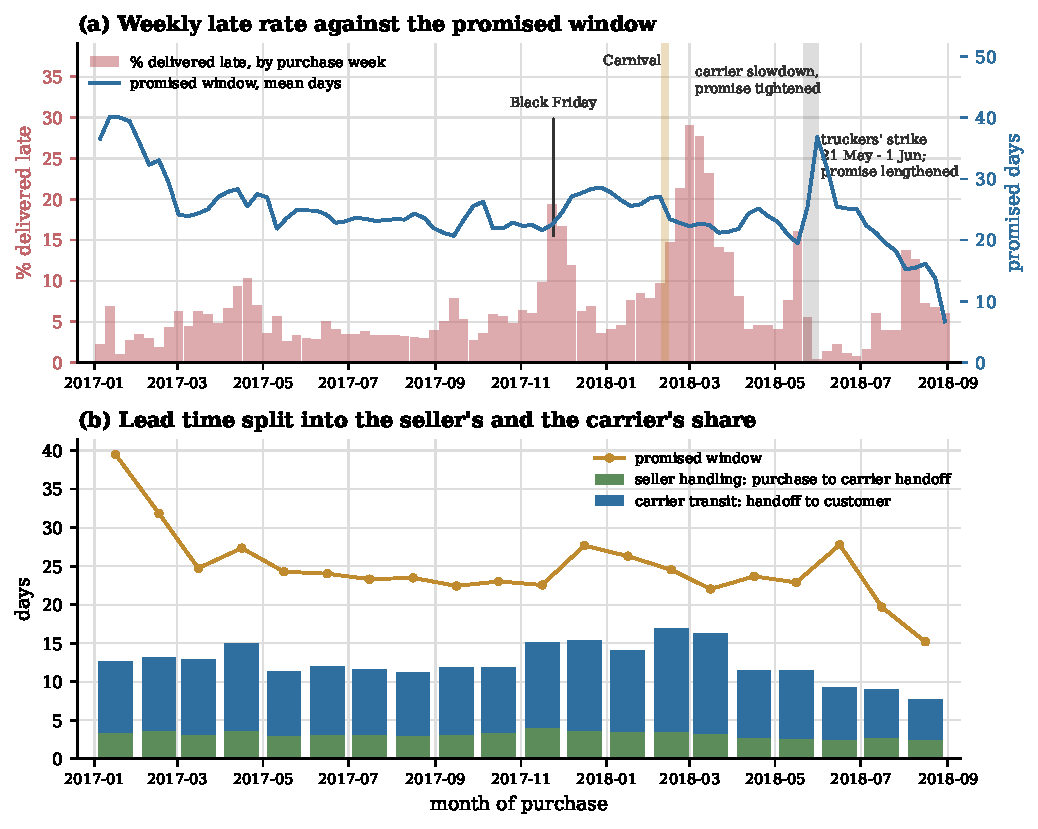
\includegraphics[width=\linewidth]{fig21_lateness_anatomy.pdf}
  \caption{Where the late deliveries came from (Appendix~\ref{app:lateness}).
  (a) Weekly late rate against the promised window: the February--March 2018
  peak coincides with a tightened promise, and the strike of 21 May--1 June 2018
  (shaded) hits the week promised before it, after which the promise is
  lengthened and the late rate collapses. (b) Lead time split at the carrier
  handoff: the peak is carrier transit, not seller handling.}
  \label{fig:lateness}
\end{figure}

\begin{figure}[htbp]
  \centering
  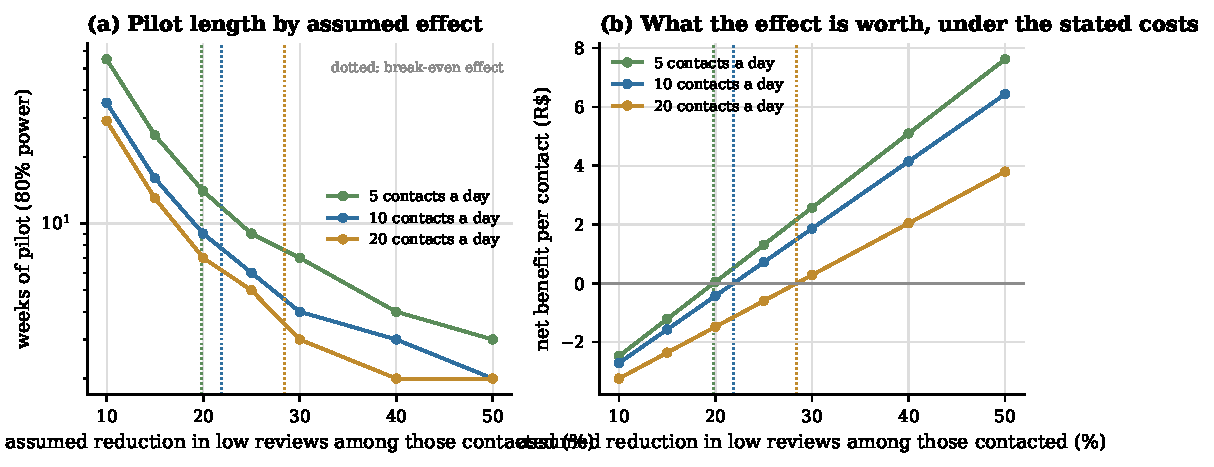
\includegraphics[width=\linewidth]{fig23_pilot.pdf}
  \caption{Sizing the outreach pilot (Section~\ref{sec:pilot}). (a) Weeks
  needed, at 80\% power, to detect a given reduction in low reviews among the
  customers contacted, for three daily capacities; the dotted lines mark each
  capacity's break-even effect. (b) The net benefit per contact that reduction
  would imply under the stated costs.}
  \label{fig:pilot}
\end{figure}

\begin{figure}[htbp]
  \centering
  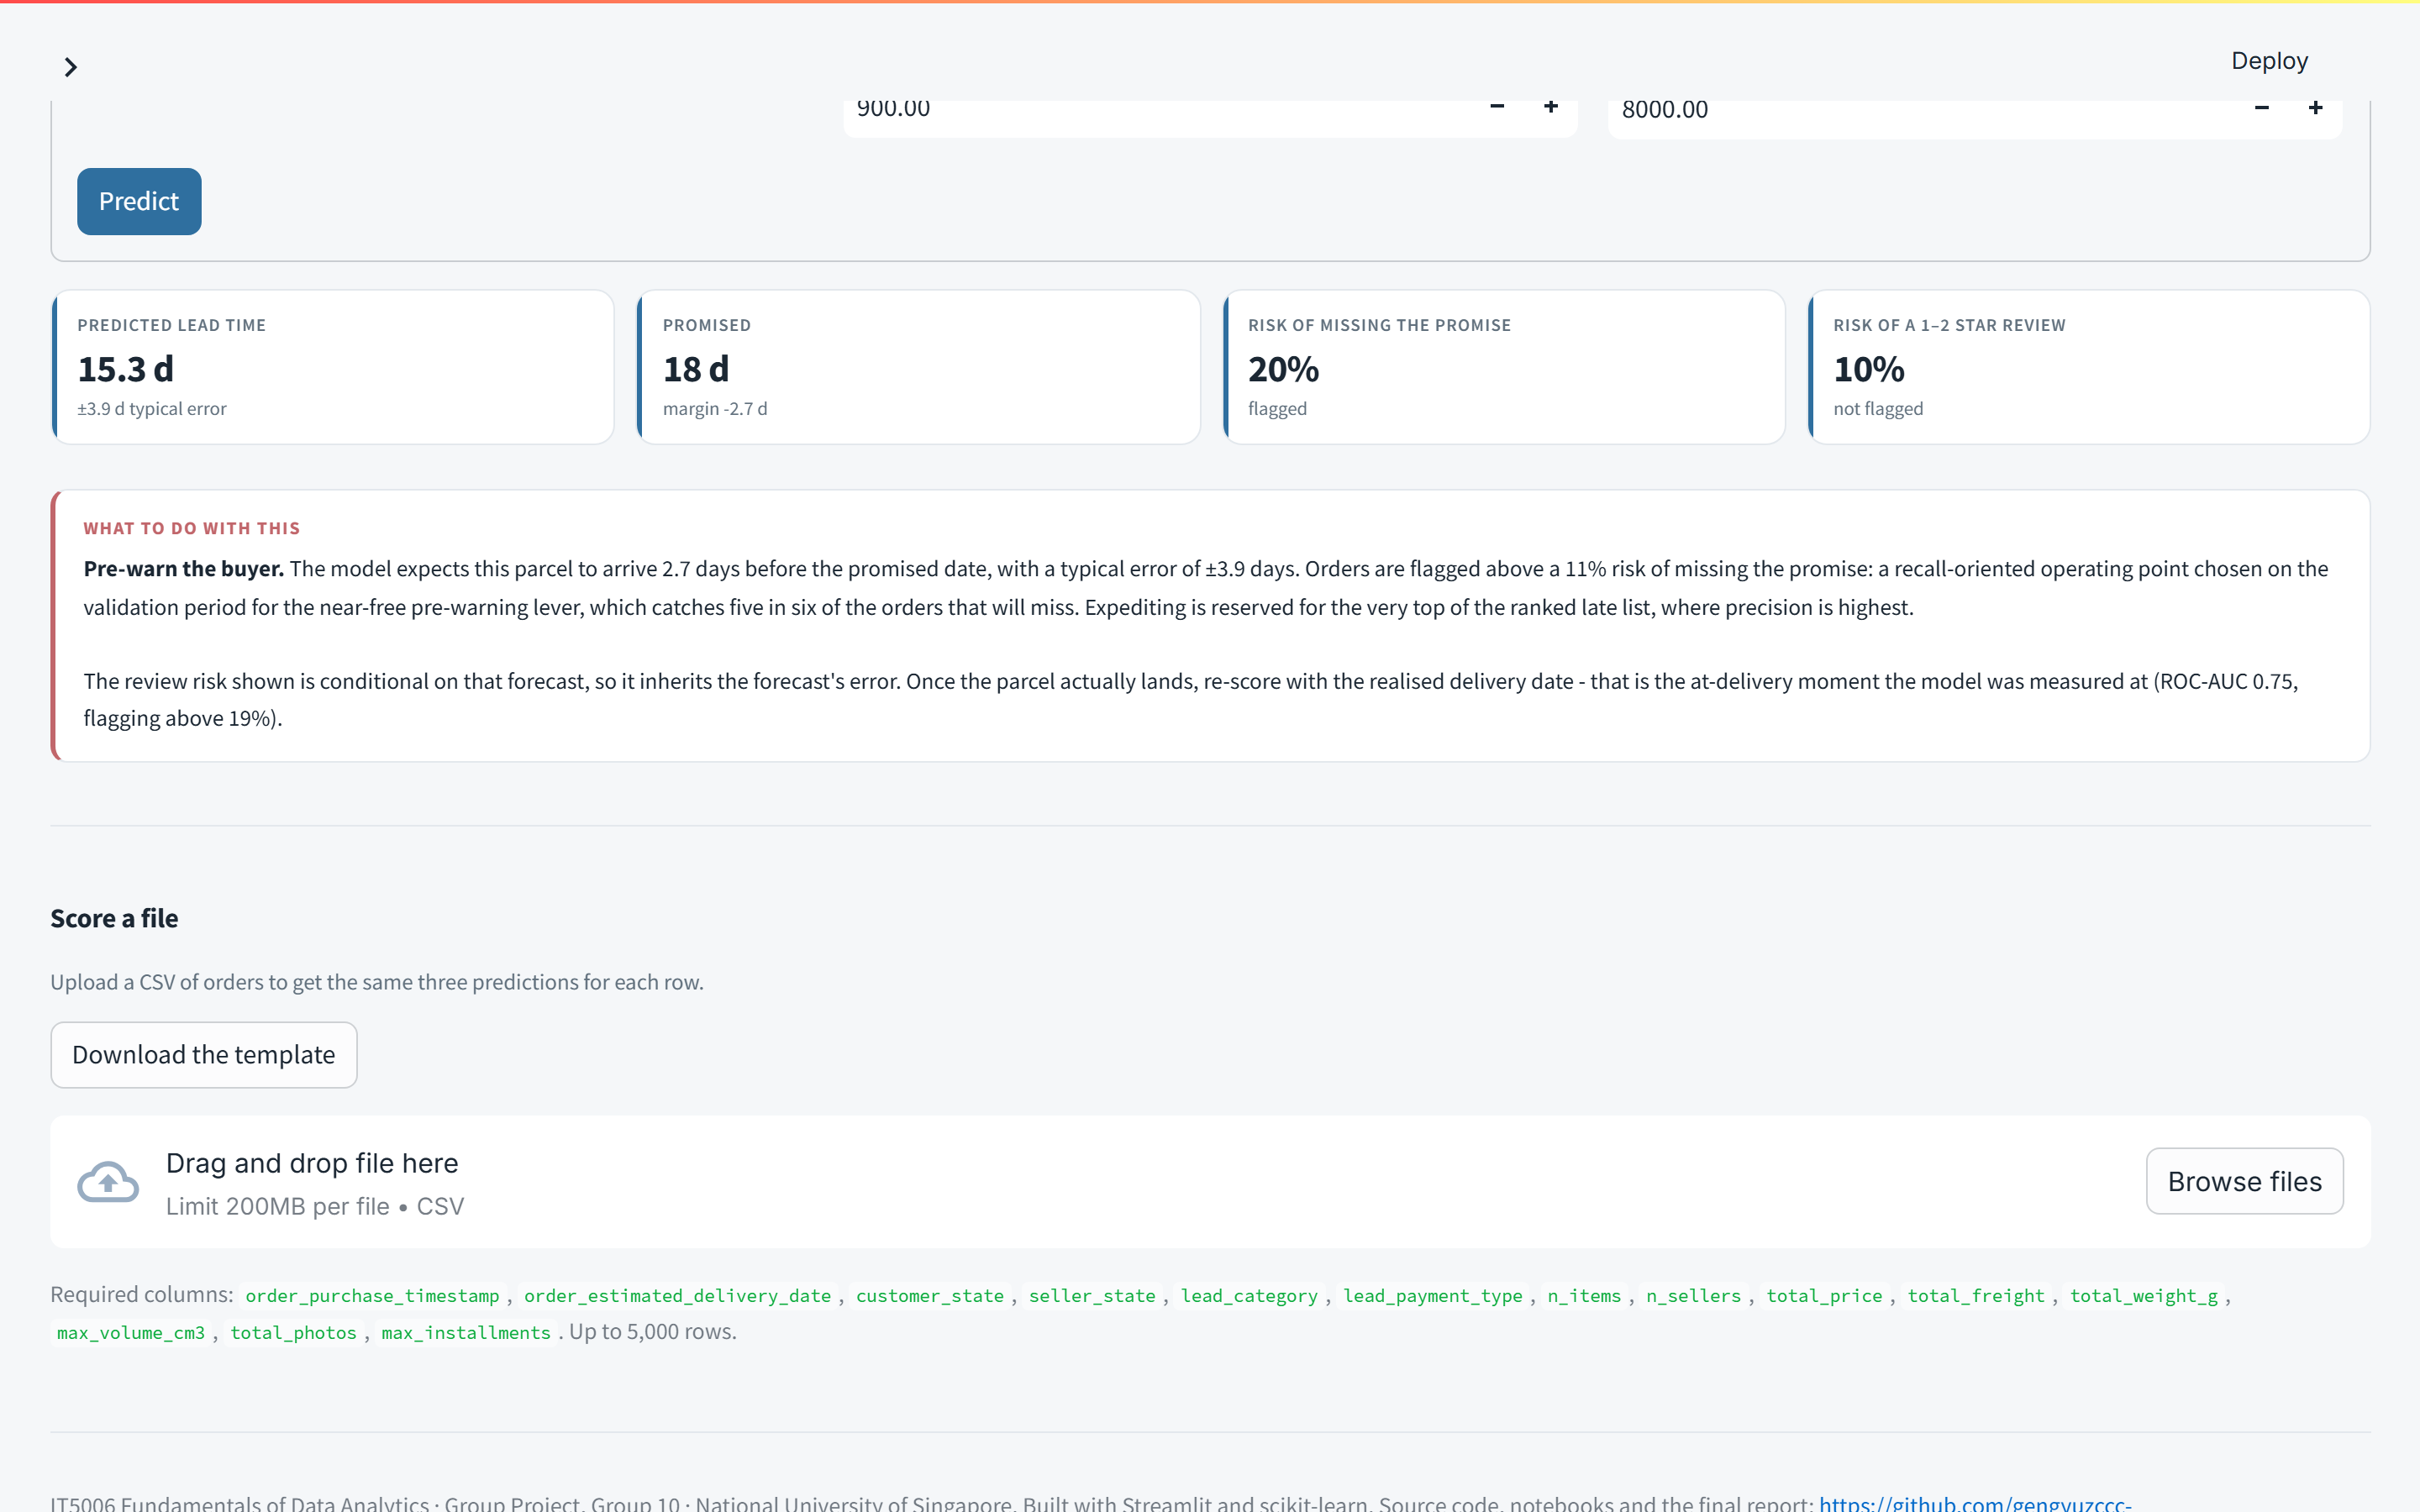
\includegraphics[width=\linewidth]{app_predict.png}
  \caption{The deployed application, Predict tab: one order scored at checkout
  --- expected lead time, the risk of missing the promise against the tuned
  threshold, and the resulting review risk --- with the batch scorer and the
  top-$K$ triage list below.}
  \label{fig:app-predict}
\end{figure}

\begin{figure}[htbp]
  \centering
  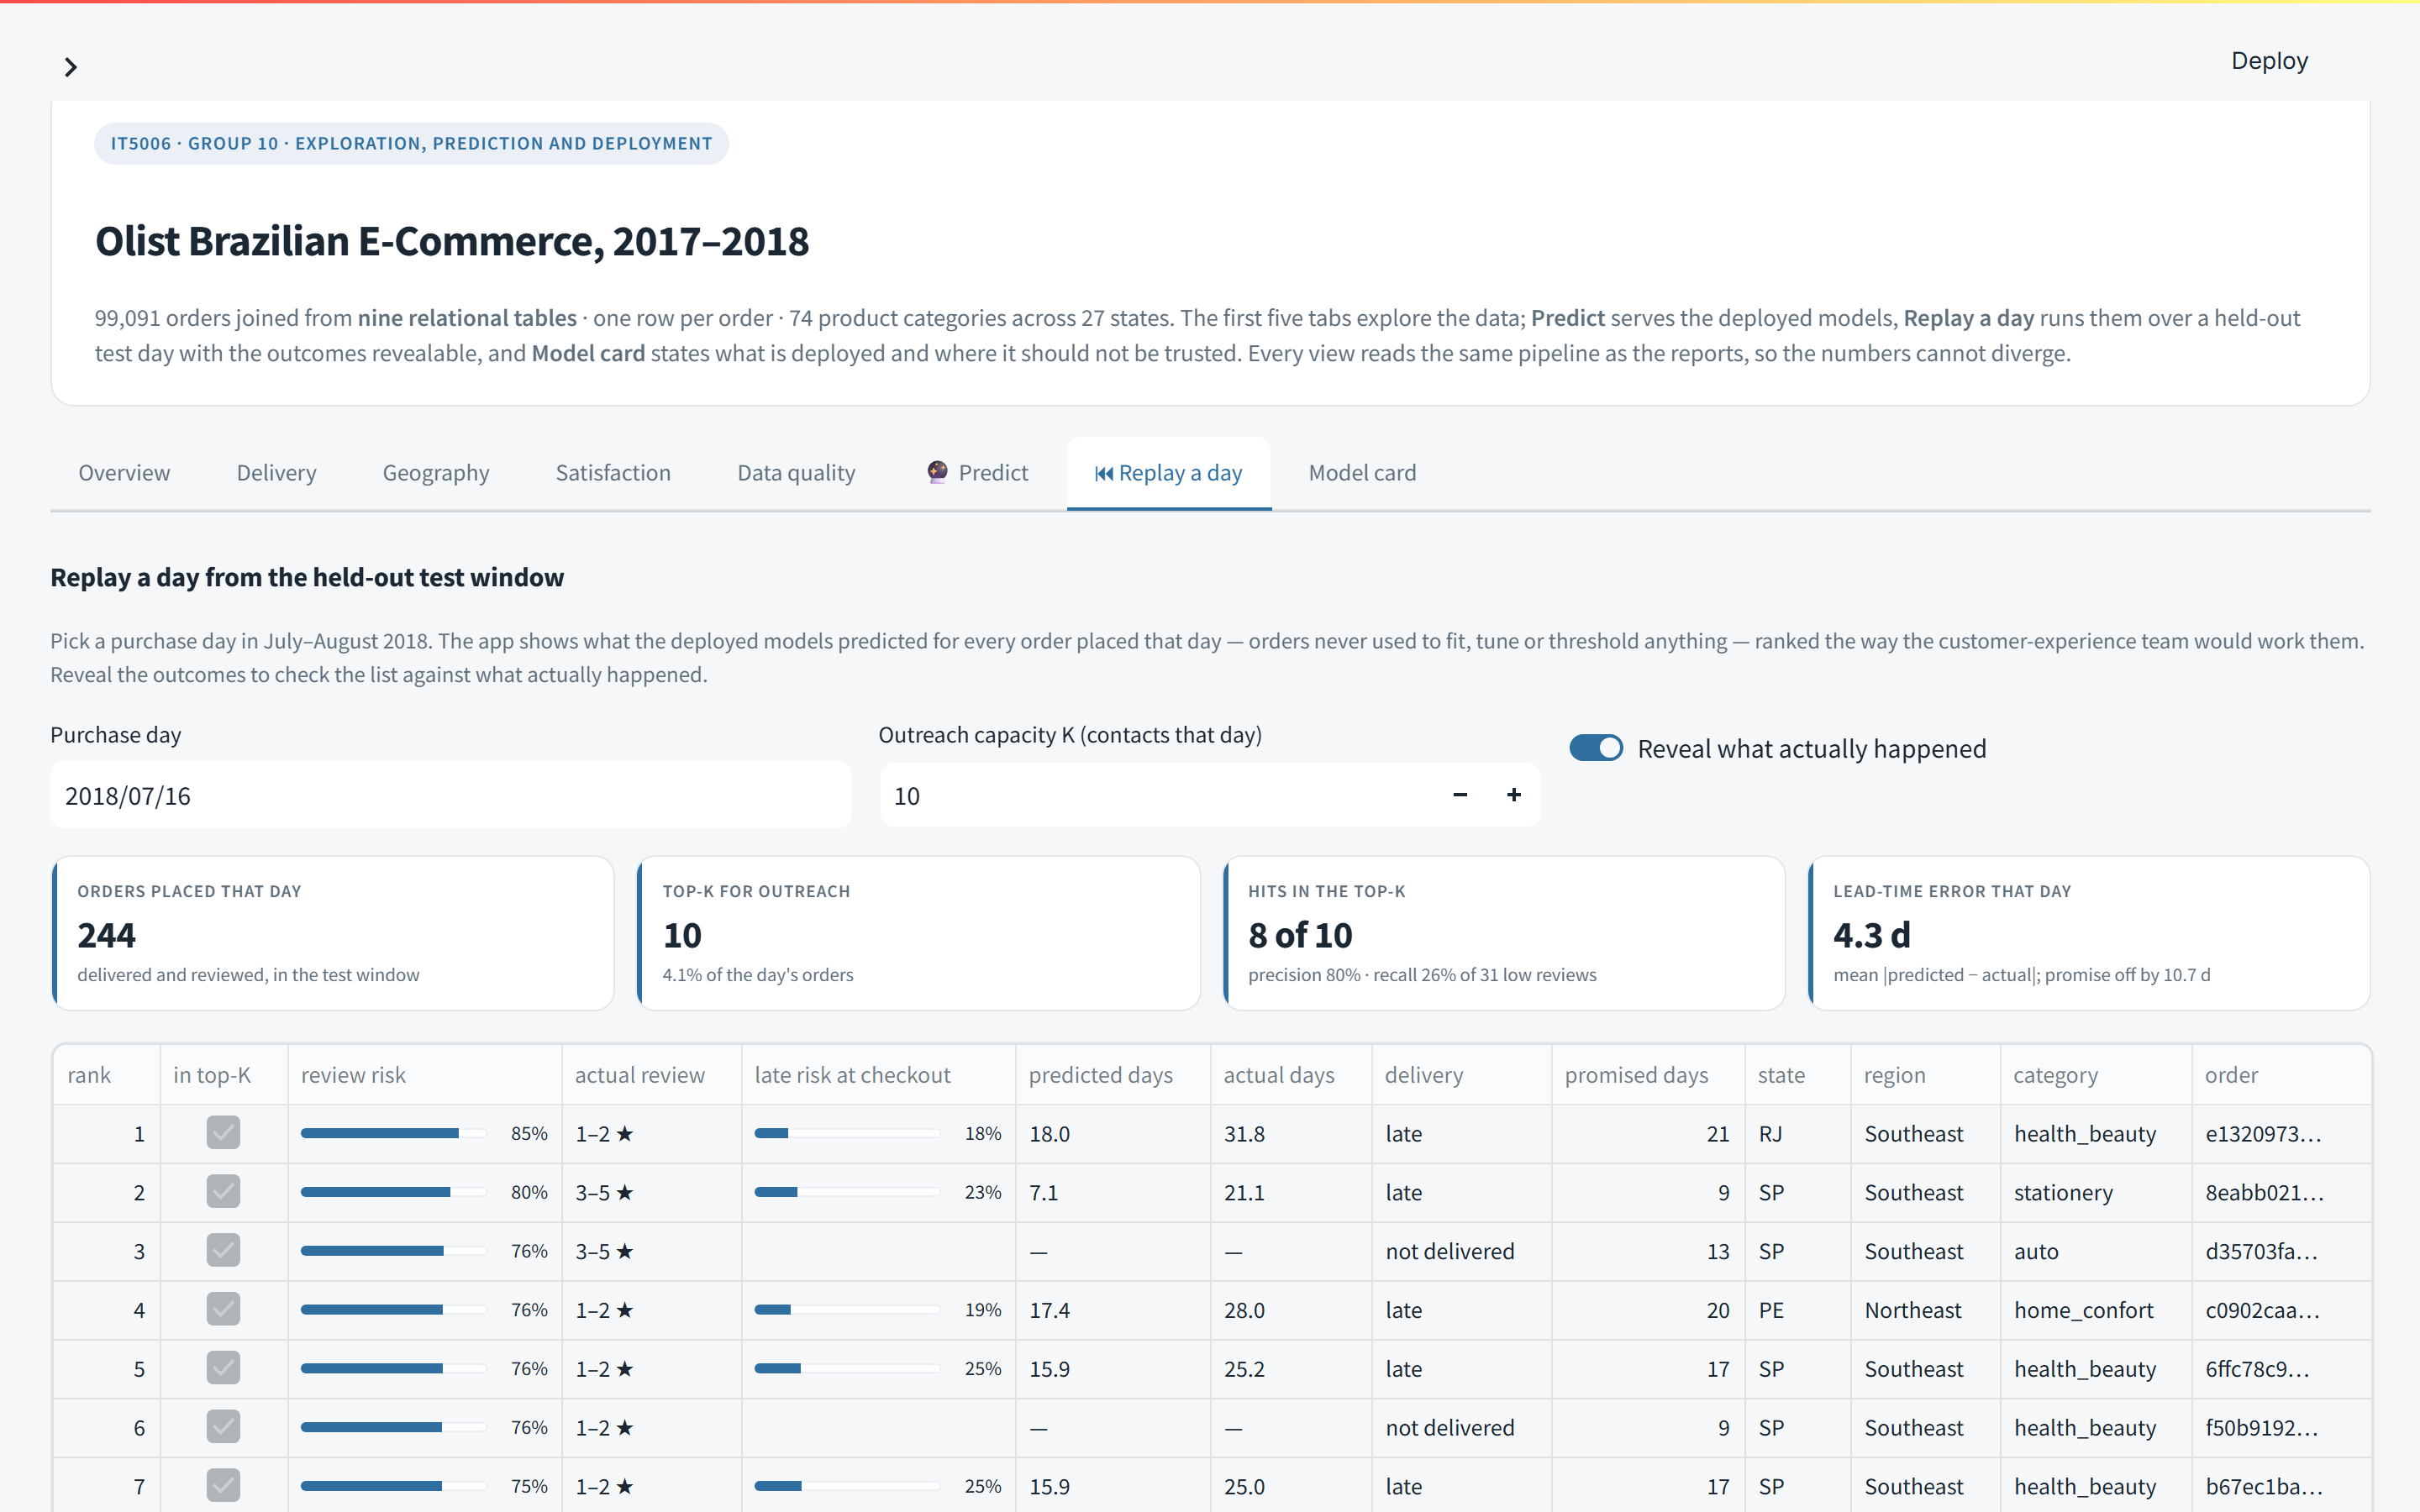
\includegraphics[width=\linewidth]{app_replay.png}
  \caption{The deployed application, Replay a day: the held-out orders placed on
  16 July 2018 ranked by review risk with a capacity of ten, outcomes revealed.
  Eight of the ten would have reached a customer who left a 1--2 star review;
  the right-hand panel shows the same capacity's precision on every day of the
  test window.}
  \label{fig:app-replay}
\end{figure}

\begin{figure}[htbp]
  \centering
  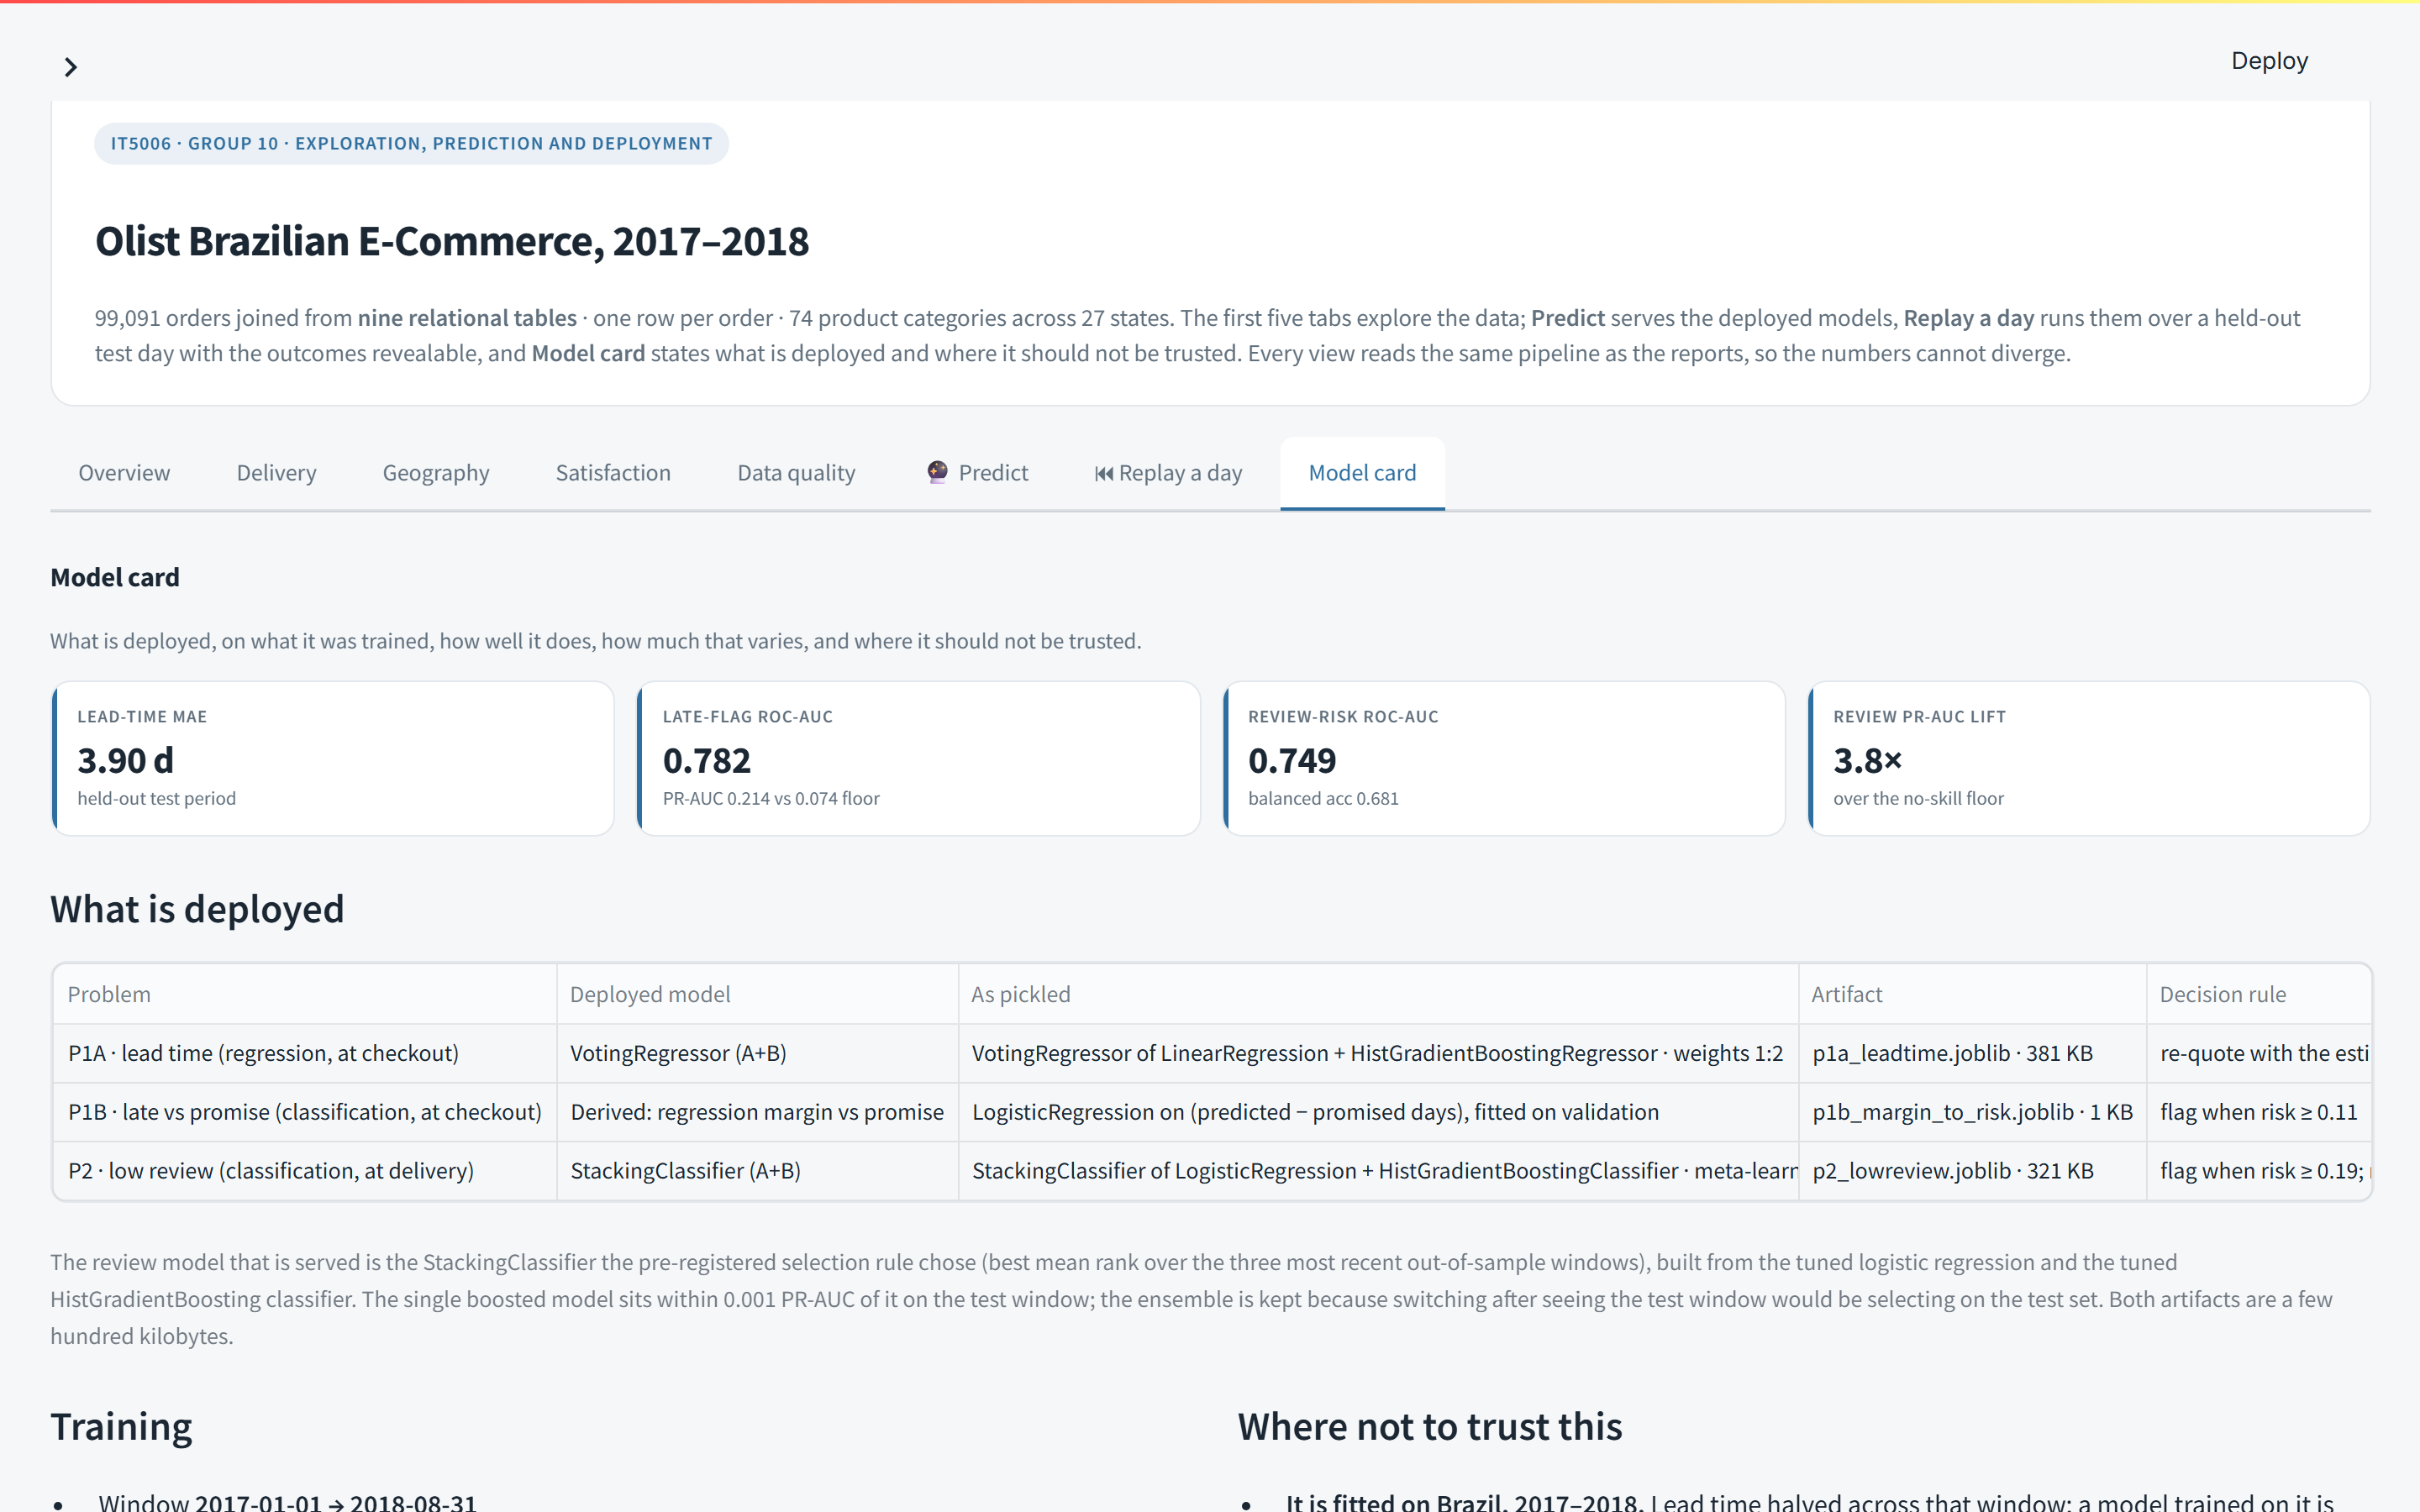
\includegraphics[width=\linewidth]{app_card.png}
  \caption{The deployed application, Model card: the estimators as pickled, the
  training protocol, where the models should not be trusted, and the
  fold-to-fold table.}
  \label{fig:app-card}
\end{figure}
